\section{Cuestionario} 
\vspace{\baselineskip}
5.1 Los valores introducidos al archivo sysctl.conf ¿que representan?

\vspace{\baselineskip}

{\bfseries fs.suid\_dumpable}
\\
\\

{\bfseries fs.aio-max-nr}
\\
\\

{\bfseries fs.file-max}
\\
\\

{\bfseries kernel.shmmni}
\\
\\

{\bfseries  kernel.sem}
\\
\\Los semáforos actúan como banderas para la memoria compartida. Los semáforos se activan o desactivan. Cuando un proceso de Oracle accede al SGA en la memoria compartida, busca un semáforo para esa porción de memoria. \\
\\
\\Los valores para los semáforos representan lo siguiente:\\
\\•	semmsl : el número de semáforos por conjunto
\\•	semmns : el número total de semáforos disponibles
\\•	semopm : el número de operaciones que se pueden realizar por llamada de semáforo
\\•	semmni : el número máximo de segmentos de memoria compartida disponibles en el sistema
\\

{\bfseries  net.ipv4.ip\_local\_port\_range}
\\
\\Define el rango de puertos locales que utilizan TCP y UDP para elegir el puerto local. El primer número es el primero, el segundo el último número de puerto local. 
\\Si es posible, es mejor que estos números tengan una paridad diferente, es decir, uno par y uno impar. 
\\

{\bfseries  net.core.rmem\_default}
\\
\\Define el rango de puertos locales que utilizan TCP y UDP para elegir el puerto local. El primer número es el primero, el segundo el último número de puerto local. 
\\Si es posible, es mejor que estos números tengan una paridad diferente, es decir, uno par y uno impar. 
\\

{\bfseries  net.core.rmem\_max}
\\
\\Esto establece el tamaño máximo del búfer de recepción del sistema operativo para todos los tipos de conexiones.
\\

{\bfseries  net.core.wmem\_default}
\\
\\Esto establece el tamaño del búfer de envío del sistema operativo predeterminado para todos los tipos de conexiones.
\\

{\bfseries  net.core.wmem\_max}
\\
\\Esto establece el tamaño del búfer de envío del sistema operativo predeterminado para todos los tipos de conexiones.
\\

\newpage

5.2 ¿Con qué usuario(s) puedo conectarme al servidor a través del Administrador
Empresarial?
	\begin{center}
		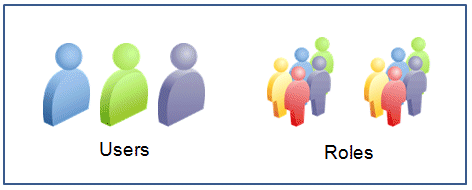
\includegraphics[width=13cm]{./Imagenes/users} 
	\end{center} 

\vspace{\baselineskip}

5.3 Capture una imagen de pantalla del navegador con el Administrador Empresarial, con el nombre de su servidor e iniciada la sesión del usuario SYS.
	\begin{center}
		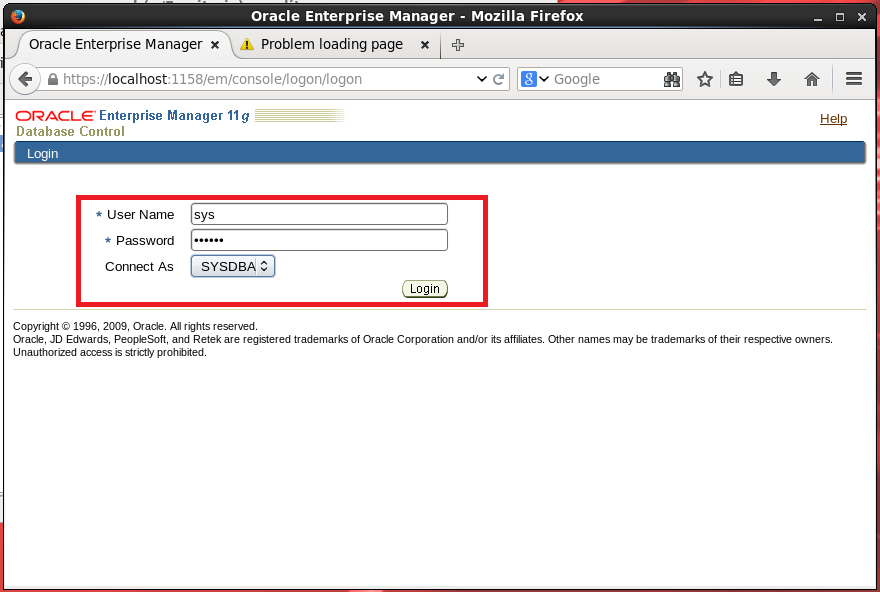
\includegraphics[width=13.2cm]{./Imagenes/92} 
	\end{center}
	
	\begin{center}
		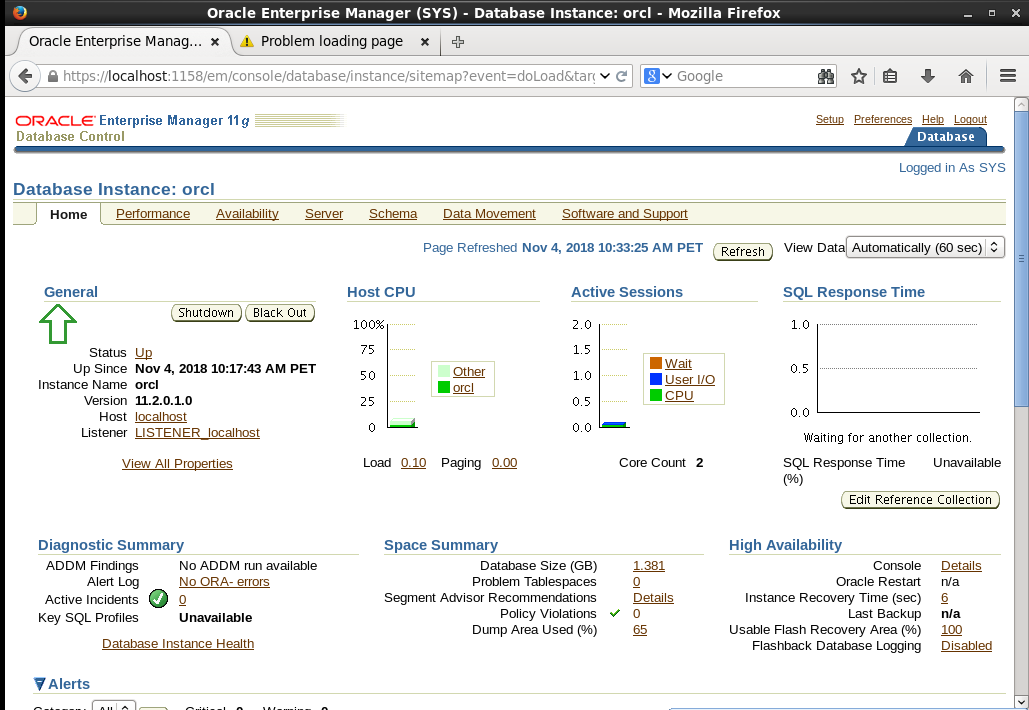
\includegraphics[width=13.2cm]{./Imagenes/93} 
	\end{center}